\section{Hybrid Programming} % using MPI+MPI$_{sm}$}

Most HPC systems in use today are clusters of shared memory nodes. The idea of hybrid programming consists of combining parallelization on the node interconnect with parallelization inside of each node. Traditionally, parallelization between nodes is being achieved using a distributed memory programming model such as MPI, while parallelization inside nodes is achieved using a shared memory programming model such as OpenMP, posix threads, or MPI$_{sm}$. 

\medskip
It has been recognized that getting good performance from a hybrid model can be difficult and requires understanding how the different programming models may interact \cite{UsingAdvancedMPI}. However, there are several reasons for using hybrid programing:

\begin{itemize} 

\item To reduce the memory footprint. Many codes require large lookup data structures that are global to the computation and ofter constant. For performance efficiency the data is ofter replicated at each process causing the memory demands of the application to grow with the number of processes. Sharing memory between MPI processes inside a node can often allow a way to share the data structure and keep only one copy per node instead of one copy per process. Nowadays this is becoming increasingly important since the number of cores in supercomputers is growing much faster than the number of nodes and than the amount of memory-per-core.

\item To reduce communication among processes. This could be achievable by directly accessing memory eliminating the need of communication through message passing between processes inside nodes.


\end{itemize}


\medskip

This section presents results of a parallel sparse matrix-vector multiplication (SPMV), a widely used operation in many simulations and the main kernel in iterative solvers, and compares its performance with and without using shared memory.


\medskip


\subsection*{Parallel SPMV}

The sparse matrix-vector multiplication (SPMV) consist in solving Equation (\ref{eq:spmv}), where A is a sparse \emph{N X N} matrix and \emph{v} is a dense \emph{N}-dimensional vector \cite{BienzGO16}.


\begin{equation}
  w = A * v
\label{eq:spmv}  
\end{equation}

In parallel, the sparse system is often distributed across processes such that each process holds a contiguous subset of rows from matrix \emph{A} and the corresponding subset of rows from vectors \emph{v} and \emph{w}. Within a single processes, it is common to splits the non-zeros values of its rows into two groups: an on-process block containing values associated to columns of the matrix that correspond to the part of vector \emph{v} values stored locally, and an off-process block containing the remainder of the non-zeros that are associated with vector \emph{v} values that are stored on other processes\cite{BienzGO16}. This is illustrated in Figure \ref{fig:Matrix}, for a case in which the matrix \emph{A} and vectors \emph{v}, \emph{w} are divided among four processes. Different colors are used to illustrate the on-process block corresponding to each process. The same color is used to show the corresponding part of vectors \emph{w} and \emph{v}. In each process the off-process values of \emph{A} occupy the remainder space, shown here without color.

\medskip

\begin{figure}[h!]
    \centering
    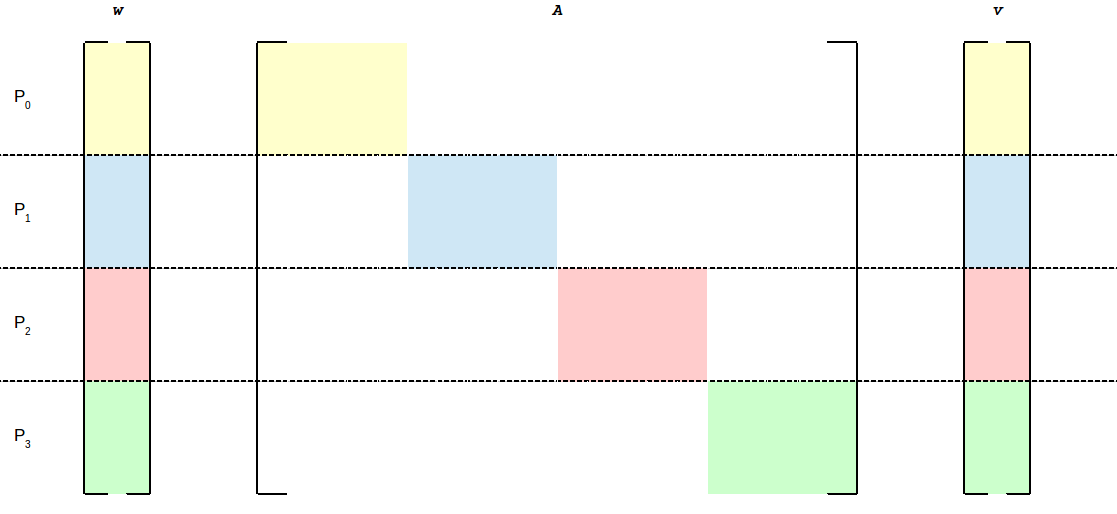
\includegraphics[width=100mm]{Plots/HybridProgramming/matrix.png}
    \caption{On-Proccess blocks shown in color.}
    \label{fig:Matrix}
\end{figure}

\medskip



With this configuration, the solution of Equation (\ref{eq:spmv}) can be obtained by executing it twice in each process. The first time using only the on-process block of matrix \emph{A} and the on-process part of the \emph{v} vector. The second time using the off-process block of matrix \emph{A} and elements of the \emph{v} vector held in other processes. These two partial solutions must be added to obtain the actual solution. Notice that while the first solution can be performed by each process independently, not requiring any communication among processes, the second solution require communication among the processes because each process requires part of the \emph{v} vector existing in other processes. For a more detailed explanation on the whole algorithm the reader could take a look at \cite{BienzGO16}.

\medskip

It is known that, as the number of processes increases, the communication time start to dominate the execution time of the kernel. This is true even when communication is carefully overlapped with communication. As stated above, the communication part of this process consist in receiving parts of the \emph{v} vector held in other processes. These parts need to be communicated, perhaps using traditional send/receive calls, even if both processes involved in the communication reside in the same node.

\medskip

The amount of communication of this kernel can be reduced if a process could have direct access to elements of the \emph{v} vector beyond those held by itself. One extreme way to achieve this is by replicating the whole \emph{v} vector in each process; that would eliminate all the required communication. However, given that the \emph{v} vector is dense, this is, in general, a prohibitive alternative. 

\medskip

Another possibility would be if all the processes residing inside a node could have direct access to the parts of the \emph{v} vector already existing in the node. Referring to Figure \ref{fig:Matrix}, assume a case in which first two processes resides in a node, $N_0$, while the last two processes resides in a different node, $N_1$. The parts of the \emph{v} vector corresponding to $P_0$ and $P_1$ are in $N_0$, but these parts are only accessible by their corresponding process. However, if these parts of the \emph{v} vector were allocated using shared memory, they would be accessed by all the processes in the node. 

\medskip

Figure \ref{fig:MatrixSm} help to illustrate the case of using shared memory for storing the \emph{v} vector. Here the shared memory is represented by the absence of separation in \emph{v} vector between the part held in $P_0$ and $P_1$ and between $P_2$ and $P_3$ as compared to Figure \ref{fig:Matrix}. Under this configuration, the processes inside a node (e.g. $P_0$ and $P_1$ in $N_0$) are able to access all the elements of the \emph{v} vector existing in that node. Additionally, the on-process block of matrix \emph{A} is expanded (and the off-process block contracted) proportionally to the number of processes existing in the node, effectively eliminating all the intra-node communication, and reducing the communication to only the inter-node part. Notice that all the part of matrix \emph{A} and of the \emph{w} vector belonging to a process are still completely hidden (not shared) form all the other processes.



\begin{figure}[t!]
    \centering
    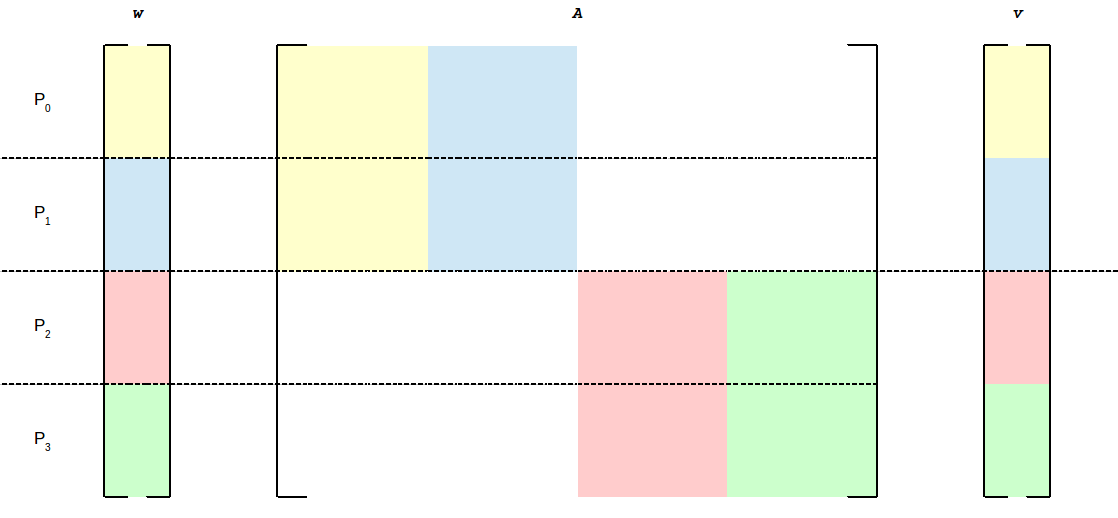
\includegraphics[width=100mm]{Plots/HybridProgramming/matrixSm.png}
    \caption{Expanded On-process blocks per process due to use of shared memory.}
    \label{fig:MatrixSm}
\end{figure}

\medskip

\subsection*{Preliminary Results}


The idea of using shared memory to reduce communication in the SPMV kernel, presented in the previous section,
was implemented in one of the SPMV functions inside Raptor, a high performance algebraic multigrid solver \cite{BiOl2017}. Preliminary results are presented in this section. 

\medskip

The following figures compare the performance of two the SPMV kernel implementations: one using traditional MPI and the other, a hybrid one, using the shared memory capabilities of MPI-3 ($MPI+MPI_{Sm}$).

\medskip

First, results obtained using individual systems (one node) are presented. For this case, all the communication among the processors is intra-node, and therefore is totally eliminated by the use of shared memory. Later, results obtained using a small 4-node cluster and Blue Waters are also presented.

\medskip

Figure \ref{fig:spmvIndividual} shows the results obtained in individual systems (one node) solving an unstructured matrix divided among sixteen processes. The figure also allows to compare the performance of the two SPMV implementations obtained using three different compilers. 


\medskip

The results obtained in individual nodes allow to see that the use of shared memory to hold the \emph{v} vector produced a performance improvement with respect to the pure MPI case in every system and compiler tested. Although the magnitude of the improvement of the $MPI+MPI_{Sm}$ version of the SMPV kernel varies among systems and compilers, it is clear that the use of shared memory to eliminate the intra-node communication is an effective mean of achieving some additional performance.




\begin{figure} [h!]
    \centering
    \captionsetup{justification=centering, singlelinecheck=false}
    \begin{subfigure}{.6\textwidth}
      \centering
      \hspace*{-1.5cm} 
      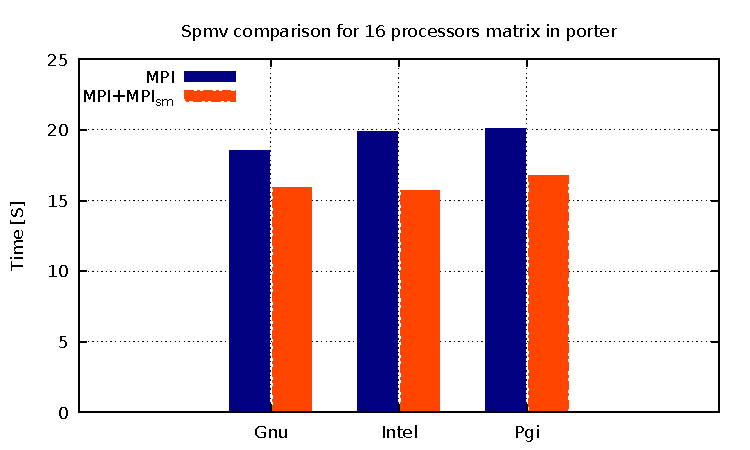
\includegraphics[page=1, width=0.95\linewidth]{Plots/HybridProgramming/spmvIndividual.pdf}
      \caption[]{Porter}
      \label{fig:HybridPorter}
    \end{subfigure}%
    \begin{subfigure}{.6\textwidth}
      \centering
      \hspace*{-1.5cm} 
      \includegraphics[page=2, width=0.95\linewidth]{Plots/HybridProgramming/spmvIndividual.pdf}
      \caption{Stout.}
      \label{fig:HybridStout}
    \end{subfigure}
    \begin{subfigure}{.6\textwidth}
      \centering
      \hspace*{-1.5cm} 
      \includegraphics[page=3, width=0.95\linewidth]{Plots/HybridProgramming/spmvIndividual.pdf}
      \caption[]{Dunkel.}
      \label{fig:HybridDunkel}
    \end{subfigure}%
    \begin{subfigure}{.6\textwidth}
      \centering
      \hspace*{-1.5cm} 
      \includegraphics[page=4, width=0.95\linewidth]{Plots/HybridProgramming/spmvIndividual.pdf}
      \caption{Koelsch.}
      \label{fig:HybridKoelsh}
    \end{subfigure}
\caption{MPI vs Hybrid $MPI+MPI_{Sm}$ SPMV comparison in individual systems.}
\label{fig:spmvIndividual}
\end{figure}


\medskip

The four systems used to obtain the results shown in Figure \ref{fig:spmvIndividual} were used together in the form of a four-node cluster, to evaluate the traditional and hybrid implementation of the SPMV kernel. Once again, three compilers were used in the evaluation. However this time, in addition of solving the previously matrix (16 processes), two other unstructured matrices were also tested: one divided among 32 processes (8 processes per node) and the other divided among 64 processes (16 processes per node). 


\begin{figure} [h!]
    \centering
    \captionsetup{justification=centering, singlelinecheck=false}
    \begin{subfigure}{.6\textwidth}
      \centering
      \hspace*{-1.5cm} 
      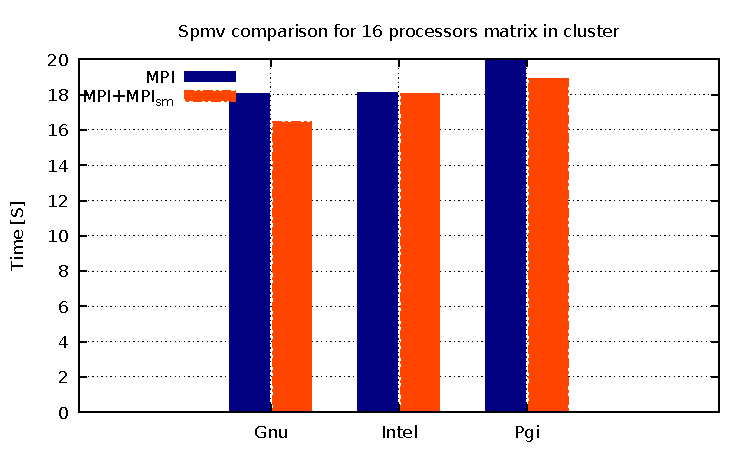
\includegraphics[page=1, width=0.95\linewidth]{Plots/HybridProgramming/spmvCluster.pdf}
      %\caption[]{Caption 1.}
      \label{fig:HybridPorter}
    \end{subfigure}%
    \begin{subfigure}{.6\textwidth}
      \centering
      \hspace*{-1.5cm} 
      \includegraphics[page=2, width=0.95\linewidth]{Plots/HybridProgramming/spmvCluster.pdf}
      %\caption{Caption 2.}
      \label{fig:HybridStout}
    \end{subfigure}
    \begin{subfigure}{.6\textwidth}
      \centering
      \hspace*{-1.5cm} 
      \includegraphics[page=3, width=0.95\linewidth]{Plots/HybridProgramming/spmvCluster.pdf}
      %\caption[]{Caption 3.}
      \label{fig:HybridDunkel}
    \end{subfigure}
\caption{MPI vs Hybrid $MPI+MPI_{Sm}$ SPMV comparison in 4-node cluster.}
\label{fig:spmvCluster4}
\end{figure}


\medskip

Figure \ref{fig:spmvCluster4} present the results obtained in the four-node cluster. Once again the hybrid version of the SPMV kernel shows different degrees of performance improvement with respect to its traditional counterpart, although the magnitude of performance improvement seems to vary depending on the matrix.

\medskip

To verify the results obtained in the 4-node cluster, the comparison of the three matrices was also done in 4 nodes of the Blue Waters supercomputer. However this test was only performed using the GNU compiler. Figure \ref{fig:spmvClusteBW} present this results. Once again, the hybrid version of the SPMV kernel always outperform the traditional one.

\medskip


\begin{figure} [h!]
    \centering
    \captionsetup{justification=centering, singlelinecheck=false}
    \begin{subfigure}{.6\textwidth}
      \centering
      \hspace*{-1.5cm} 
      \includegraphics[page=4, width=0.95\linewidth]{Plots/HybridProgramming/spmvCluster.pdf}
      %\caption[]{Blue Waters}
      \label{fig:HybridPorter}
    \end{subfigure}%
\caption{MPI vs Hybrid $MPI+MPI_{Sm}$ SPMV comparison in 4 Blue Waters nodes using the Gnu Compiler.}
\label{fig:spmvClusteBW}
\end{figure}




\subsection*{Summary}

The sparse matrix-vector multiplication represented by Equation \ref{eq:spmv} was used to compare a traditional (non-hybrid) parallel implementation with a hybrid one in which the \emph{v} vector was allocated using shared memory, effectively given access to it to all the processes co-existing in a node. Although the memory footprint was not changed, a reduction in the amount of communication required by the algorithm produce an increment of performance.


